\documentclass[a4paper]{article}
\usepackage[utf8]{inputenc}
\usepackage[spanish, es-tabla, es-noshorthands]{babel}
\usepackage[table,xcdraw]{xcolor}
\usepackage[a4paper, footnotesep = 1cm, width=20cm, top=2.5cm, height=25cm, textwidth=18cm, textheight=25cm]{geometry}
%\geometry{showframe}

\usepackage{tikz}
\usepackage{amsmath}
\usepackage{amsfonts}
\usepackage{amssymb}
\usepackage{float}
\usepackage{graphicx}
\usepackage{caption}
\usepackage{subcaption}
\usepackage{multicol}
\usepackage{multirow}
\setlength{\doublerulesep}{\arrayrulewidth}
\usepackage{booktabs}

\usepackage{hyperref}
\hypersetup{
    colorlinks=true,
    linkcolor=blue,
    filecolor=magenta,      
    urlcolor=blue,
    citecolor=blue,    
}

\newcommand{\quotes}[1]{``#1''}
\usepackage{array}
\newcolumntype{C}[1]{>{\centering\let\newline\\\arraybackslash\hspace{0pt}}m{#1}}
\usepackage[american]{circuitikz}
\usetikzlibrary{calc}
\usepackage{fancyhdr}
\usepackage{units} 

\graphicspath{{../Ejercicio-1/}{../Ejercicio-2/}}

\pagestyle{fancy}
\fancyhf{}
\lhead{22.67 - Señales Aleatorias}
\rhead{Lambertucci, Londero B., Moriconi, Musich, Tolaba}
\rfoot{Página \thepage}
\begin{document}
\subsection{Introducción}

El siguiente ejercicio parte de un análisis sobre el proceso aleatorio presente en la página 138 del libro selecto por la cátedra. Se realizarán simulaciones de dicho proceso y se calcularán experimentalmente la media, la varianza, la autocorrelación y el coeficiente de autocorrelación para ciertos valores de t dados y se realizará una comparación con los valores teóricos.
Luego, se.... PUNTO C 

\subsection{Valores teóricos}

El experimento que determina el proceso es la tirada de un dado no cargado y el ensamble del mismo se detalla a continuación:

\begin{center}		%Estaria bueno alinear esto pero no se como 
	 $y_{1} = 6$\\
	 $y_{2} = 3sin(t)$\\
	 $y_{3} = -3sin(t)$\\
	 $y_{4} = 3cos(t)$\\
	 $y_{5} = -3cos(t$)\\
	 $y_{6} = -6$\\
\end{center}

El proceso es $Y_{(t)} = y_{i(t)}$ donde i indica el número obtenido en la tirada del dado.

El valor esperado del proceso teóricamente se obtiene de la siguiente forma:

\begin{equation*}
\begin{gathered}
	E\left[Y_{(t)}\right] = \sum_{i=1}^{6}\left( P(Y_{(t)} = y_{i(t)}) \times y_{i(t)}\right) 
\end{gathered}
\end{equation*}

Reemplazando las funciones muestra dadas y que la probabilidad $P(Y_{(t)} = y_{i(t)})= \frac{1}{6}$ $ \forall i $ obtenemos que:

\begin{equation*}
\begin{gathered}
	E\left[Y_{(t)}\right] = 0$ $\forall t 
\end{gathered}
\end{equation*}

La varianza se obtiene como

\begin{equation*}
\begin{gathered}
	\sigma^{2}_{(t)} = E\left[Y_{(t)}^{2}\right]- \left(E\left[Y_{(t)}\right]\right)^{2}  
\end{gathered}
\end{equation*}

Donde ya se obtuvo que $E\left[Y_{(t)}\right] = 0$ y 

\begin{equation*}
\begin{gathered}
	E\left[Y_{(t)}^{2}\right] = \sum_{i=1}^{6}\left( P(Y_{(t)} = y_{i(t)}) \times y_{i(t)}^{2}\right) 
\end{gathered}
\end{equation*}

Finalmente
\begin{equation*}
\begin{gathered}
	\sigma^{2}_{(t)} = 15 $   $ \forall t  
\end{gathered}
\end{equation*}

Este proceso tiene media y varianza constantes para todo instante t.

La autocorrelaci[on para dos instantes t1 y t2


El coeficiente de autocorrelaci[on 


\subsection{Análisis Experimental}

Para el análisis sobre los valores pedidos es necesario generar múltiples muestras sobre el proceso, en los instantes de tiempo requeridos. En primer lugar, se obtiene un número entero al azar entre 1 y 6, simulando la tirada de un dado, el cual determina qué función miembro del ensamble resulta.
A partir de la determinacion de la función correspondiente se evalua en los valores de instantes t pedidos, obteniendose:

\begin{enumerate}
   \item[•] $Y(\pi/2)$
   \item[•] $Y(\pi/4)$
   \item[•] $Y(\pi)$
   \item[•] $Y(2\pi)$
\end{enumerate}

Estos valores obtenidos se guardan como un vector. Luego, se repite el procedimiento N = 1000 veces 
y se obtiene un arreglo de vectores conteniendo muestras del proceso.
El codigo de Matlab empleado para la simulaci[on de este proceso se detalla a continuaci[on 
\\

\begin{figure}[H]
\centering
	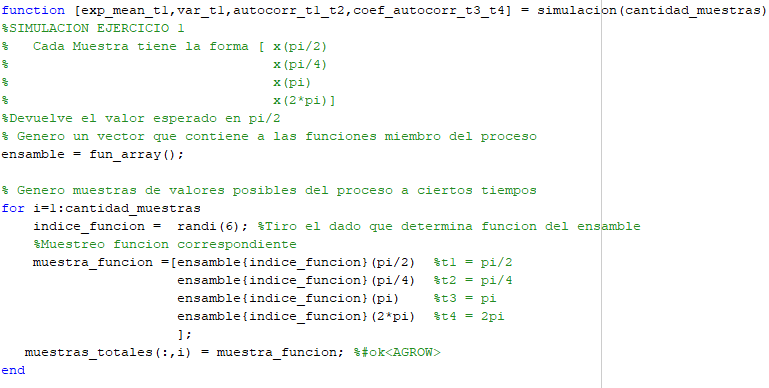
\includegraphics[width=0.8\textwidth, trim = {0 0 0 0},clip]{./ImagenesEjercicio1/main1.png}
	\caption{.}
	\label{fig:main1}
\end{figure}

Donde la funcion fun-array() designa el ensamble solicitado, el c[odigo en Matlab:

\begin{figure}[H]
\centering
	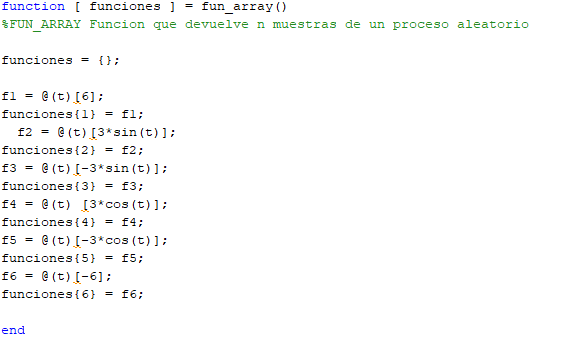
\includegraphics[width=0.6\textwidth, trim = {0 0 0 0},clip]{./ImagenesEjercicio1/fun_array.png}
	\caption{.}
	\label{fig:fun_array}
\end{figure}

A continuación, por ejemplo se muestran los resultados para $Y(\pi/2)$ para N = 100 experimentos realizados.

\begin{figure}[H]
\centering
	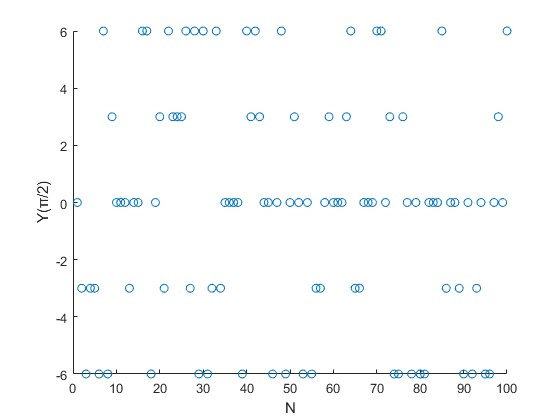
\includegraphics[width=0.4\textwidth, trim = {0 0 0 0},clip]{./ImagenesEjercicio1/ypi_2.png}
	\caption{.}
	\label{fig:ypi_2}
\end{figure}

Tambi[en para $Y(\pi/4)$.

\begin{figure}[H]
\centering
	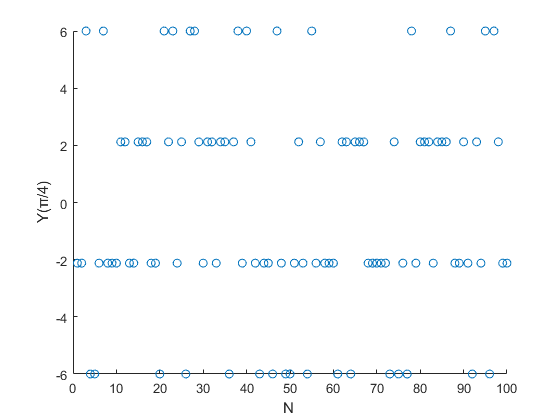
\includegraphics[width=0.4\textwidth, trim = {0 0 0 0},clip]{./ImagenesEjercicio1/ypi_4.png}
	\caption{.}
	\label{fig:ypi_4}
\end{figure}

Observaci[on: En las Figuras (\ref{fig:ypi_2}) y (\ref{fig:ypi_4})se puede "estimar" visualmente que la media para el proceso es cero. 
\\
Luego, se calculan promediando los valores pedidos con el c[odigo:

\begin{figure}[H]
\centering
	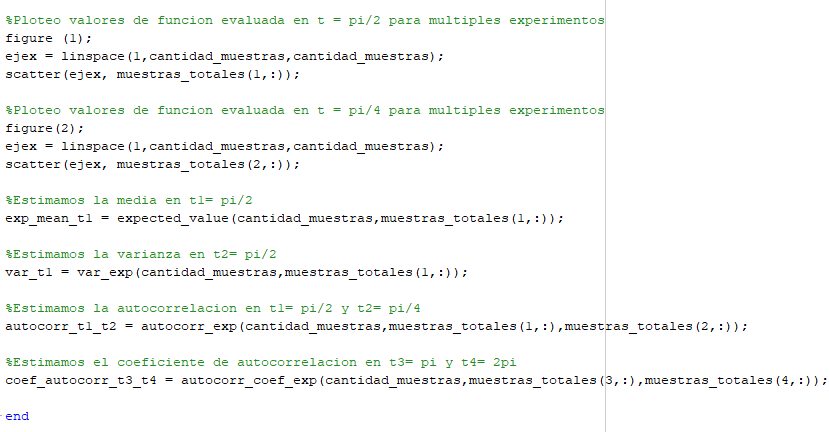
\includegraphics[width=0.8\textwidth, trim = {0 0 0 0},clip]{./ImagenesEjercicio1/main2.png}
	\caption{.}
	\label{fig:main2}
\end{figure}

Detallando cada funci[on:
\begin{enumerate}
\item[•] La funcio[n estimadora de la media en $t = \frac{\pi}{2}$, E$\left[ Y_{(\frac{\pi}{2})}\right]$
\begin{figure}[H]
\centering
	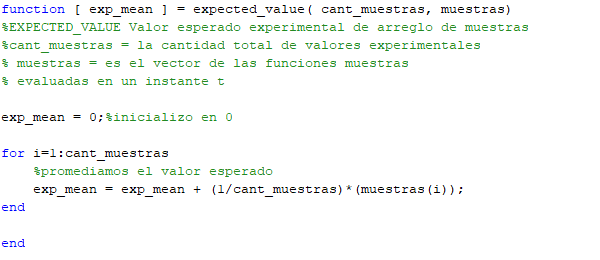
\includegraphics[width=0.6\textwidth, trim = {0 0 0 0},clip]{./ImagenesEjercicio1/expval.png}
	\caption{.}
	\label{fig:expval}
\end{figure}

\item[•] La funci[on estimadora de la varianza en $t = \frac{\pi}{2}$, Var$\left[Y_{(\frac{\pi}{2})}\right]$
\begin{figure}[H]
\centering
	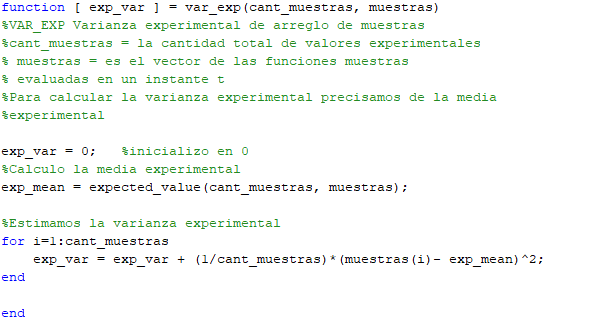
\includegraphics[width=0.6\textwidth, trim = {0 0 0 0},clip]{./ImagenesEjercicio1/expvar.png}
	\caption{.}
	\label{fig:expvar}
\end{figure}

\item[•] La funci[on estimadora de la autocorrelacio[n en $t_1 = \frac{\pi}{4}$ y $t_2 = \frac{\pi}{2}$, $R_{xx(\frac{\pi}{4},\frac{\pi}{2})}$
\begin{figure}[H]
\centering
	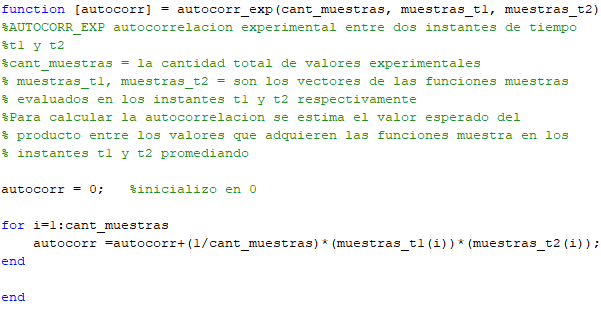
\includegraphics[width=0.6\textwidth, trim = {0 0 0 0},clip]{./ImagenesEjercicio1/autocorr.png}
	\caption{.}
	\label{fig:autocorr}
\end{figure}

\item[•] La funci[on estimadora del coeficiente de autocorrelacio[n en $t_3 = \frac{2\pi}{4}$ y $t_4 = \pi$, $r_{xx(2\pi,\pi)}$
\begin{figure}[H]
\centering
	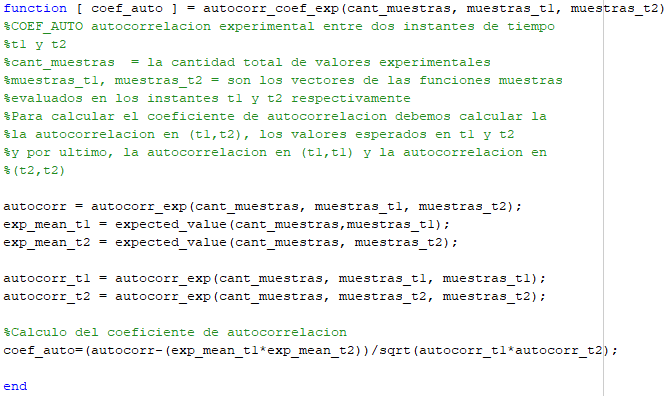
\includegraphics[width=0.6\textwidth, trim = {0 0 0 0},clip]{./ImagenesEjercicio1/coefauto.png}
	\caption{.}
	\label{fig:coefauto}
\end{figure}
\end{enumerate}
\\
Corriendo 



\end{document}